\documentclass[11pt]{article}
\usepackage{graphicx}
\usepackage{tcolorbox}
\usepackage{amsmath}
\usepackage{multicol}
\usepackage{amssymb}
\usepackage{amsthm}
\usepackage{amsfonts}
\usepackage{float}
\usepackage[font=small,skip=0pt]{caption}
\makeatletter
\captionsetup[figure]{skip=0pt}
\title{\vspace{-5.0cm}KTH Royal Institute of Technology\\ DD2424-VT19-1 Deep Learning in Data Science\\ Assignment 1 }
\author{Marina Herrera Sarrias }

\begin{document}
\maketitle

\section{Exercise 1} Images corresponding to the following parameter settings:

\subsection{\texttt{lambda=0, n\_epochs=40, n\_batch=100, eta=.1}}\label{1.1}


\begin{figure}[H]
	\centerline{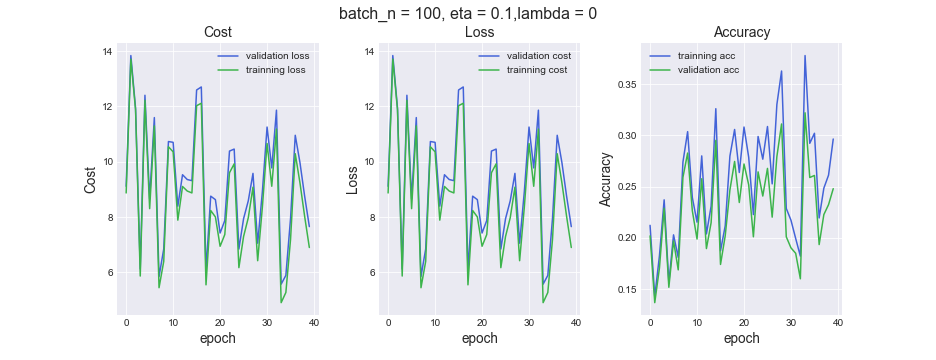
\includegraphics[width=195mm,scale=0.7]{lamda_0_eta_01.png}}
	\caption{The graph of the training and validation cost, loss and accuracy computed after every epoch. The network was trained with the following parameter settings$:$ \texttt{n\_batch}$=100$ \texttt{eta}$=0.1$, \texttt{n\_epochs}$=40$ and  \texttt{lambda}$=0$.}
	\label{fig:1}
\end{figure}

\begin{figure}[H]
	\centerline{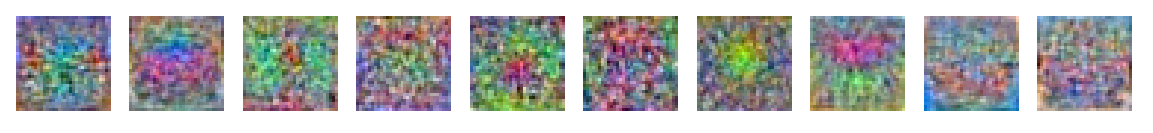
\includegraphics[width=195mm,scale=0.7]{lamda_0_eta_01_ct.png}}
	\caption{The graph of the training and validation cost, loss and accuracy computed after every epoch. The network was trained with the following parameter settings$:$ \texttt{n\_batch}$=100$ \texttt{eta}$=0.1$, \texttt{n\_epochs}$=40$ and  \texttt{lambda}$=0$.}
	\label{fig:1.1}
\end{figure}
\subsection{\texttt{lambda=0, n\_epochs=40, n\_batch=100, eta=.01}}\label{1.2}

\begin{figure}[H]
	\centerline{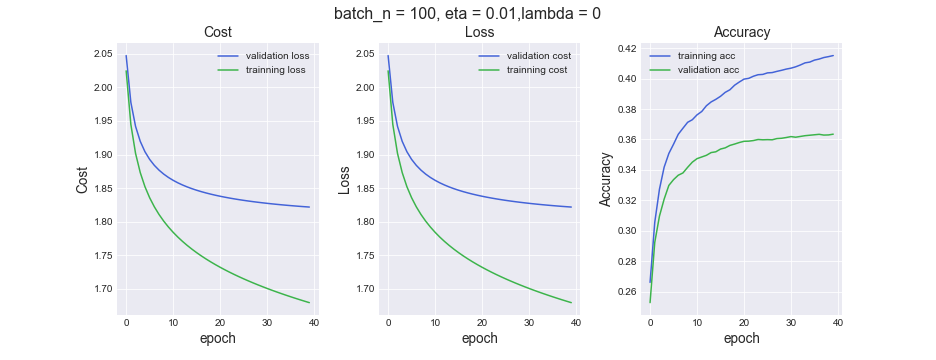
\includegraphics[width=195mm,scale=0.7]{lamda_0_eta_001.png}}
		\caption{The graph of the training and validation cost, loss and accuracy computed after every epoch. The network was trained with the following parameter settings$:$ \texttt{n\_batch}$=100$ \texttt{eta}$=.01$, \texttt{n\_epochs}$=40$ and  \texttt{lambda}$=0$.}
	\label{fig:2}
\end{figure}

\begin{figure}[H]
	\centerline{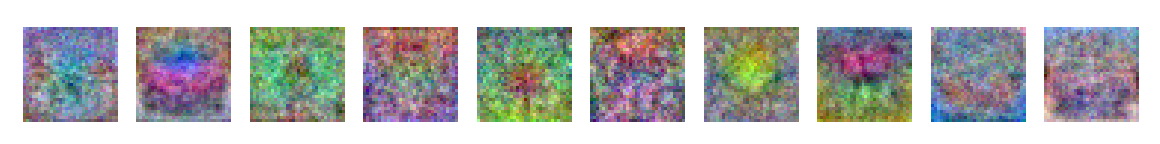
\includegraphics[width=200mm,scale=0.5]{lamda_0_eta_001_ct.png}}
	\caption{The graph of the training and validation cost, loss and accuracy computed after every epoch. The network was trained with the following parameter settings$:$ \texttt{n\_batch}$=100$ \texttt{eta}$=.01$, \texttt{n\_epochs}$=40$ and  \texttt{lambda}$=0$.}
	\label{fig:2.1}
\end{figure}

\subsection{\texttt{lambda=.1, n\_epochs=40, n\_batch=100, eta=.01}}\label{1.3}
\begin{figure}[H]
	\centerline{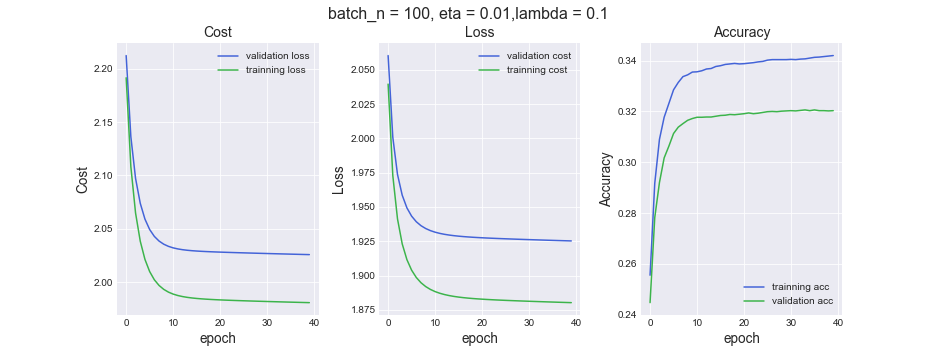
\includegraphics[width=195mm,scale=0.7]{lamda_01_eta_001.png}}
	\caption{The graph of the training and validation cost, loss and accuracy computed after every epoch. The network was trained with the following parameter settings$:$ \texttt{n\_batch}$=100$ \texttt{eta}$=.01$, \texttt{n\_epochs}$=40$ and  \texttt{lambda}$=0.1$.}
	\label{fig:3}
\end{figure}

\begin{figure}[H]
	\centerline{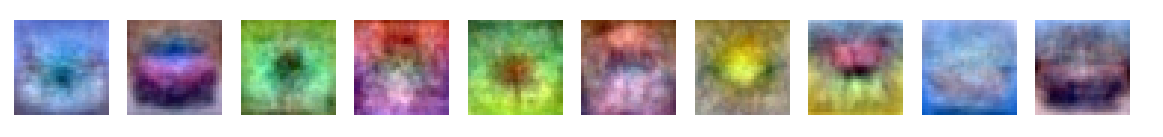
\includegraphics[width=200mm,scale=0.5]{lamda_01_eta_001_ct.png}}
	\caption{The learnt W matrix visualized as class template images. The network was
		trained with the following parameter settings: \texttt{n\_batch}$=100$, \texttt{eta}$=.01$, \texttt{n\_epochs}$=40$
		and \texttt{lambda}$=0.1$.}
	\label{fig:3.1}
\end{figure}

\subsection{\texttt{lambda=1, n\_epochs=40, n\_batch=100, eta=.01}}\label{1.4}

\begin{figure}[H]
	\centerline{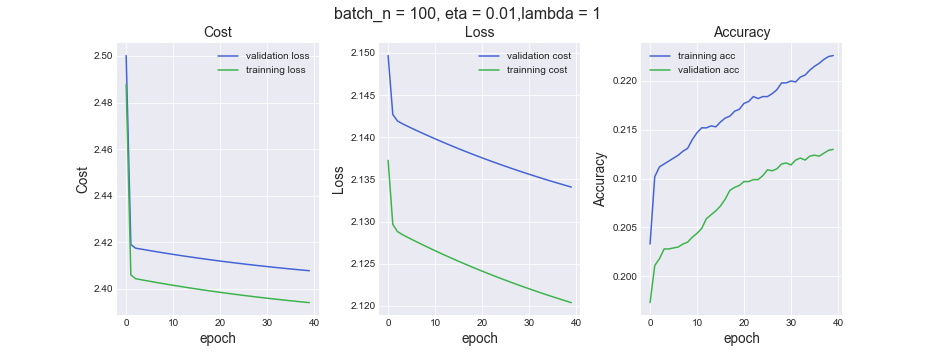
\includegraphics[width=195mm,scale=0.7]{lamda_1_eta_001.png}}
	\caption{The graph of the training and validation cost, loss and accuracy computed after every epoch. The network was trained with the following parameter settings$:$ \texttt{n\_batch}$=100$ \texttt{eta}$=.01$, \texttt{n\_epochs}$=40$ and  \texttt{lambda}$=1$.}
	\label{fig:4}
\end{figure}

\begin{figure}[H]
	\centerline{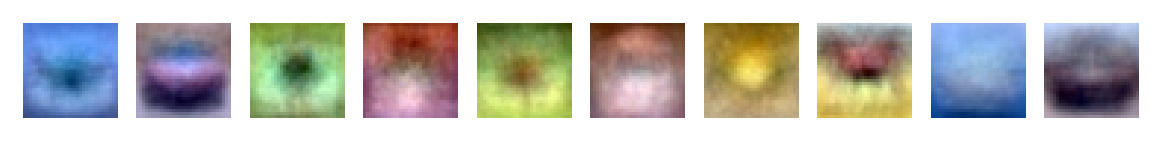
\includegraphics[width=195mm,scale=0.5]{lamda_1_eta_001_ct.png}}
	\caption{The learnt W matrix visualized as class template images. The network was
	trained with the following parameter settings: \texttt{n\_batch}$=100$, \texttt{eta}$=.01$, \texttt{n\_epochs}$=40$
	and \texttt{lambda}$=1$.}
	\label{fig:4.1}
\end{figure}

After training the networks for the different  parameter settings using mini-batch gradient descent, we can conclude that the training with minimum validation cost and maximum accuracy is given by the parameter settings in section  \ref{1.2}, achieving a maximum accuracy of  $36.51\%$. \\

In none of the cases above, adding regularization improved the accuracy of the network. As the value of \texttt{lambda} increased from $0.1$ (Figure.\ref{fig:3}) to $1$ (Figure.\ref{fig:4}), the network's accuracy decreased. Furthermore, we can also say that adding the term does not improve the minimization of the cost function, in both cases the loss decreased more than the actual cost, implying that adding regularization does not contribute to the cost minimization of the model. \\

Finally, the best performance was achieved on the setting with lower learning rate (\texttt{eta}$=.01$). When the value of \texttt{eta} is set too high, such as in Figure (\ref{fig:1}) the learning rate causes instability and fails to converge. While on the other hand, when the value of \texttt{eta} is set too low it will take longer to converge, if it ever does. Furthermore, in both of the cases mentioned before, a "bad" value of \texttt{eta} leads to an increase on the training error.\\

The learning rate controls how quickly or slowly our network learns, therefore, it is one of the most important hyper-parameters to tun in our model. There is not a possible way to calculate the best learning rate for a given model and data-set. Therefore we will need to find it. A grid search can help us to find a fixed learning rate while a method like applying a learning rate decay can make our model to learn faster. I will discuss both techniques on the bonus assignment.\\

I verified the analytical computations of the gradients using numerical estimations. With the finite difference formula I obtained $2.33\text{e-}07$ as the maximum relative error for both gradients $W$ and $b$. While using the centered difference formula I obtained $7.21\text{e-}08$ as the maximum relative error for the $W$ gradients and $1.32\text{e-}09$ for $b$. We can verify that the Central difference provides more accuracy in approximating to the analytical computations of the gradients.
\end{document}
